\subsection{The resulting STP}

Start by noting that constraint (\ref{P'-sjtj}) is always true and can be omitted.
Moreover, (\ref{P'-tjsj}) can be rewritten as (\ref{P'-pp}), to obtain the following reformulation:
\begin{align}
	\tag{$P'$}
	\min_{s\geq 0} \quad 	& \sum_{j\in V} \sum_{p\in \z{P}} \max(0, s_{jp} - \tau_j)		& \\
	\textrm{s.t.}\quad	&	s_{ip} - s_{jp} \leq - d_{ip}	& (i,j) \in E, p \in \z{P} \label{P'-sisj} \\
						&	s_{jp'} - s_{jp} \leq w		& (p, p') \in \z{P}^2, j\in V \label{P'-pp}
\end{align}
Those familiar with \emph{Temporal Constraint Satisfaction Problems} (TCSPs) \cite{dechter1991} will 
recognize (\ref{P'-sisj}) and (\ref{P'-pp}) as the constraints of a \emph{Simple Temporal Problem} (STP) 
with variables $T=\{s_{jp}: j \in V, p\in \z{P}\}$.
Note that if the original task network $G(V,E)$ is acyclic, the resulting STP is always \emph{consistent} (i.e. has a solution).%
\footnote{If $G(V,E)$ is acyclic, there exists an infinite number of feasible solutions $(s,t)$ for $(P)$,
for each of which there exists a counterpart $(s',t')\in \Lambda^*$ (according to Lemma~\ref{lemm-Lambda}) 
with $s'$ satisfying (\ref{P'-sisj}) and (\ref{P'-pp}).}%
The \emph{earliest-start-time assignment} (est-assignment) is a feasible solution that can be found efficiently
for a given STP by computing all-pairs-shortest-paths in its \emph{distance-graph} representation (see Fig.~\ref{fig-STN}).
In our case, variables $\{s_{1p}: p \in P\}$ can be fixed to zero, assuming that source task 1 starts at time zero in all scenarios.

\begin{figure}
	\centering
		\begin{subfigure}[b]{0.4\textwidth}
		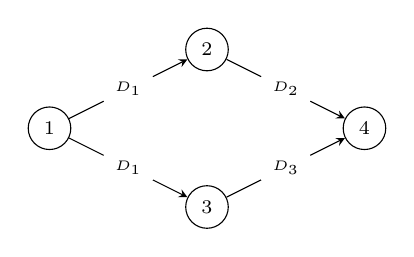
\begin{tikzpicture}
			\begin{scope}[every node/.style={circle,thin,draw}]
				\node (1a) at (+0+0,+0+0)	{\scriptsize $1$};
				\node (2a) at (+2+0,+1+0)	{\scriptsize $2$};
				\node (3a) at (+2+0,-1+0)	{\scriptsize $3$};
				\node (4a) at (+4+0,-0+0)	{\scriptsize $4$};
				
			\end{scope}

			\begin{scope}[>={stealth[black]},
				every node/.style={fill=white,circle},
				every edge/.style={draw=black,thin}]
				\path [->] (1a) edge node {\tiny $D_{1}$} (2a);
				\path [->] (1a) edge node {\tiny $D_{1}$} (3a);
				\path [->] (2a) edge node {\tiny $D_{2}$} (4a);
				\path [->] (3a) edge node {\tiny $D_{3}$} (4a);			
 			\end{scope}
		\end{tikzpicture}
		\subcaption{}
		\label{fig-STN}
	\end{subfigure}
	~
	\begin{subfigure}[b]{0.4\textwidth}
\begin{tikzpicture}
			\begin{scope}[->,>=stealth',shorten >=1pt,auto,
                semithick, scale = 1, transform shape,
                every node/.style={circle,thin,draw}]
				\node (z) at (-1.5,+1.5)	{\scriptsize $z$};
				
				\node (1a) at (+0+0,+0+0)	{\scriptsize $s_{1p}$};
				\node (2a) at (+2+0,+1+0)	{\scriptsize $s_{2p}$};
				\node (3a) at (+2+0,-1+0)	{\scriptsize $s_{3p}$};
				\node (4a) at (+4+0,-0+0)	{\scriptsize $s_{4p}$};
				
				\node (1b) at (+0+0.0,+0+3.0)	{\scriptsize $s_{1p'}$};
				\node (2b) at (+2+0.0,+1+3.0)	{\scriptsize $s_{2p'}$};
				\node (3b) at (+2+0.0,-1+3.0)	{\scriptsize $s_{3p'}$};
				\node (4b) at (+4+0.0,-0+3.0)	{\scriptsize $s_{4p'}$};				
			\end{scope}

			\begin{scope}[>={stealth[black]},
				every node/.style={fill=white,circle},
				every edge/.style={draw=black,thin}]
				
				% z1 arcs
				\path [<-] (z) edge[bend right=15] node {\tiny $0$} (1a);
				\path [->] (z) edge[bend left=15] node {\tiny $0$} (1a);
				\path [<-] (z) edge[bend right=15] node {\tiny $0$} (1b);
				\path [->] (z) edge[bend left=15] node {\tiny $0$} (1b);	
						
				% ij arcs for scenario p
				\path [<-] (1a) edge node {\tiny $-d_{1p}$} (2a);
				\path [<-] (1a) edge node {\tiny $-d_{1p}$} (3a);
				\path [<-] (2a) edge node {\tiny $-d_{2p}$} (4a);
				\path [<-] (3a) edge node {\tiny $-d_{3p}$} (4a);
				
				% ij arcs for scenario p'
				\path [<-] (1b) edge node {\tiny $-d_{1p'}$} (2b);
				\path [<-] (1b) edge node {\tiny $-d_{1p'}$} (3b);
				\path [<-] (2b) edge node {\tiny $-d_{2p'}$} (4b);
				\path [<-] (3b) edge node {\tiny $-d_{3p'}$} (4b);	

							
				% s1p - w - s1p'
				\path [->] (1a) edge[bend right=8] node[] {\tiny $w$} (1b);
				\path [<-] (1a) edge[bend left=8] node[] {\tiny $w$} (1b);
				
				% s2p - w - s2p'
				\path [dotted,<->] (2a) edge[bend left=15] node[pos=0.7] {\tiny $w$} (2b);
				
				% s3p - w - s3p'
				\path [dotted,<->] (3a) edge[bend right=15] node[pos=0.3] {\tiny $w$} (3b);
				
				% s4p - w - s4p'
				\path [->] (4a) edge[bend right=8] node[] {\tiny $w$} (4b);
				\path [<-] (4a) edge[bend left=8] node[] {\tiny $w$} (4b);
			\end{scope}
		\end{tikzpicture}
		\subcaption{}
		\label{fig-STN}
	\end{subfigure}

	\caption{The solution-space of $(P')$ is equivalent to that of a STP with a time-variable
	$s_{ip}$ for each task $i$ and scenario $p$ and constraints (\ref{P'-sisj}) and (\ref{P'-pp}).
	We illustrate here how each precedence-constraint $(i,j)$ translates to a corresponding structure in the resulting STP,
	assuming three scenarios $P=\{p,p', p''\}$ are possible.}
\end{figure}

In the est-assignment, each variable (i.e. each $s_{jp}$ in our case) takes the minimum value that it may take in a feasible solution.
As such, it clearly optimizes the objective of $(P)$ and $(P')$.
By Lemma~\ref{lemm-Lambda}, the est-assignment $s$ can be extended to an optimal olution $(s,t)$ for $(P)$ by letting 
$t_j = \max_{p\in P} s_{jp} - w$ for all $j\in V$.
An all-pairs-shortest-path algorithm such as Floyd-Warshall \cite{} takes $O(N^3)$ where $N=n m$ is the number of variables.
Therefore, we have so far managed to improve the worst-case bound of optimally trading-off tardiness and stability, 
from $O(n^5m^4)$ to $O(n^3m^3)$, which is still disappointing.
Fortunately, as we show in the following, by exploiting the special structure of the resulting STP 
we are able to compute its est-assignment in time $O(n^2m)$.
 
%
% how to convert the distance graph to a directed graph
%

If there is a path from $i$ to $j$ in $G(V, E)$,
then there is no path from $s_{ip}$ to $s_{jp'}$ for some $p, p' \in \z{P}$ in the distance-graph of the resulting STP,
but there is a path from $s_{jp'}$ to $s_{ip}$, for all $p, p' \in \z{P}$.

The distance from some $s_{jp}$ to some $s_{jp''}$ via some $s_{jp'}$ with $p\neq p' \neq p''$ is greater (by $w$)
than the distance from $s_{jp}$ to $s_{jp''}$ directly.